%%%%%%%%%%%%%%%%%%%%%%%%%%%%%%%%%%%%%%%%%
% baposter Landscape Poster
% LaTeX Template
% Version 1.0 (11/06/13)
%
% baposter Class Created by:
% Brian Amberg (baposter@brian-amberg.de)
%
% This template has been downloaded from:
% http://www.LaTeXTemplates.com
%
% License:
% CC BY-NC-SA 3.0 (http://creativecommons.org/licenses/by-nc-sa/3.0/)
%
%%%%%%%%%%%%%%%%%%%%%%%%%%%%%%%%%%%%%%%%%

%----------------------------------------------------------------------------------------
%	PACKAGES AND OTHER DOCUMENT CONFIGURATIONS
%----------------------------------------------------------------------------------------

\documentclass[landscape,a1paper,fontscale=0.5]{baposter} % Adjust the font scale/size here

\usepackage{graphicx} % Required for including images
\graphicspath{{figures/}} % Directory in which figures are stored

\usepackage{amsmath} % For typesetting math
\usepackage{amssymb} % Adds new symbols to be used in math mode

\usepackage{booktabs} % Top and bottom rules for tables
\usepackage{enumitem} % Used to reduce itemize/enumerate spacing
\usepackage{palatino} % Use the Palatino font
\usepackage[font=small,labelfont=bf]{caption} % Required for specifying captions to tables and figures
\usepackage{nth}

\usepackage{multicol} % Required for multiple columns
\setlength{\columnsep}{1.5em} % Slightly increase the space between columns
\setlength{\columnseprule}{0mm} % No horizontal rule between columns

\usepackage{tikz} % Required for flow chart
\usetikzlibrary{shapes,arrows} % Tikz libraries required for the flow chart in the template

\newcommand{\compresslist}{ % Define a command to reduce spacing within itemize/enumerate environments, this is used right after \begin{itemize} or \begin{enumerate}
\setlength{\itemsep}{1pt}
\setlength{\parskip}{0pt}
\setlength{\parsep}{0pt}
}

\definecolor{lightblue}{rgb}{0.145,0.6666,0.9} % Defines the color used for content box headers
\definecolor{black}{rgb}{0.3,0.3,0.3}
\begin{document}

\begin{poster}
{
headerborder=closed, % Adds a border around the header of content boxes
colspacing=0.7em, % Column spacing
bgColorOne=white, % Background color for the gradient on the left side of the poster
bgColorTwo=white, % Background color for the gradient on the right side of the poster
borderColor=lightblue, % Border color
headerColorOne=black, % Background color for the header in the content boxes (left side)
headerColorTwo=lightblue, % Background color for the header in the content boxes (right side)
headerFontColor=white, % Text color for the header text in the content boxes
boxColorOne=white, % Background color of the content boxes
textborder=roundedleft, % Format of the border around content boxes, can be: none, bars, coils, triangles, rectangle, rounded, roundedsmall, roundedright or faded
eyecatcher=true, % Set to false for ignoring the left logo in the title and move the title left
headerheight=0.08\textheight, % Height of the header
headershape=roundedright, % Specify the rounded corner in the content box headers, can be: rectangle, small-rounded, roundedright, roundedleft or rounded
headerfont=\Large\bf\textsc, % Large, bold and sans serif font in the headers of content boxes
%textfont={\setlength{\parindent}{1.5em}}, % Uncomment for paragraph indentation
linewidth=1.5pt, % Width of the border lines around content boxes
columns =3
}
%----------------------------------------------------------------------------------------
%	TITLE SECTION 
%----------------------------------------------------------------------------------------
%
{
\includegraphics[height=7em]{wits.jpg}} % First university/lab logo on the left
{\bf\textsc{An investigational study into the design of a low cost, adaptive hearing aid}\vspace{0.3em}} % Poster title
{\textsc{ Kayla-Jade Butkow \& Kelvin da Silva \hspace{12pt} {\small School of Electrical \& Information Engineering, University of the Witwatersrand}}} % Author names and institution
{
\includegraphics[height=7em]{EIE.pdf}} % Second university/lab logo on the right

%----------------------------------------------------------------------------------------
%	INTRODUCTION
%----------------------------------------------------------------------------------------

%\headerbox{Introduction}{name=introduction,column=0,row=0}{
%
%Hearing loss is a prevalent problem that affects people in all parts of the world. It is caused by many factors including age, disease and trauma, and often results in a decreased quality of life~\cite{Evaluation_of_a_hearing_compensation_algorithm}. Existing hearing aids are expensive, which makes them inaccessible to the majority of South Africans. It is therefore necessary to develop an inexpensive hearing aid that has all of the functionality of a high-end hearing aid.
%
%This functionality includes:
%\begin{itemize}\compresslist
%	\vspace{-0.7em}
%	\item Amplifying specific frequency bands according to a person's audiogram
%	\item The ability of the user to select the direction in which they wish to listen and to hear sounds in that direction louder than other directions
%\end{itemize}
%}

%----------------------------------------------------------------------------------------
%	OBJECTIVES
%----------------------------------------------------------------------------------------

\headerbox{Objectives}{name=objectives,column=0,row=0}{
To develop an inexpensive hearing aid that has all of the functionality of a high-end hearing aid, including:
\begin{itemize}\compresslist
	\vspace{-0.4em}
	\item Amplifying specific frequency bands according to a person's audiogram
	\item The ability of the user to select the direction in which they wish to listen and to hear sounds in that direction louder than other directions
\end{itemize}

This will be done in the form of:
\begin{itemize}\compresslist
		\vspace{-0.4em}
		\item A full software hearing aid simulation
		\item A hardware proof of concept of a hearing aid which demonstrates limited functionality
\end{itemize}
}

%----------------------------------------------------------------------------------------
%	FUTURE WORK
%----------------------------------------------------------------------------------------
\headerbox{Results: Hardware}{name=results3,column=2,row=0}{
The error in the directionality feature was calculated by comparing the measured and the simulated polar plots for each steerable angle. Compensatory gain error was calculated using the difference between the desired and measured gain at the centre of each frequency band
\begin{center}
	\captionof{table}{Average error in the directionality feature}
	\resizebox{0.3\columnwidth}{!}{%
\begin{tabular}{cc}
	\toprule
	\textbf{Angle${}^o$} & \textbf{Average Error (\%)} \\
	\midrule 
	0 & 46.6 \\ 
	60 & 30.7 \\ 
	90 & 12.7 \\ 
	120 & 22.7 \\ 
	180 & 51.7 \\ 
	\bottomrule
\end{tabular} 
	}
\end{center}

\begin{center}
	\captionof{table}{Error in the compensatory gain feature}
	\resizebox{0.5\columnwidth}{!}{%
		\begin{tabular}{cc}
			\toprule
			\textbf{Compensated frequency band (Hz)} &\textbf{Error (\%)} \\ 
			\midrule
			2820 - 3550 & 0.81 \\ 
			5620 - 7080 & 19.56 \\ 
			\bottomrule
		\end{tabular} 
	}
\end{center}
}

\headerbox{Future Work}{name=FutureWork,column=2,below=results3}{
For future development of the hearing aid, a number of improvements could be made including:
\begin{itemize}\compresslist
	\item Making use of higher quality omni-directional microphones
	\item Creating an integrated circuit chip to handle the preprocessing of the audio signals
	\item Making use of more microphones to improve the precision of the directionality feature
	\item Emdedding the microphones and circuitry into headphones to reduce the size of the device
\end{itemize}
}


%----------------------------------------------------------------------------------------
%	METHODOLOGY
%----------------------------------------------------------------------------------------

\headerbox{System Design}{name=method,column=0,below=objectives, above=bottom}{ % This block's bottom aligns with the bottom of the conclusion block

\begin{center}
	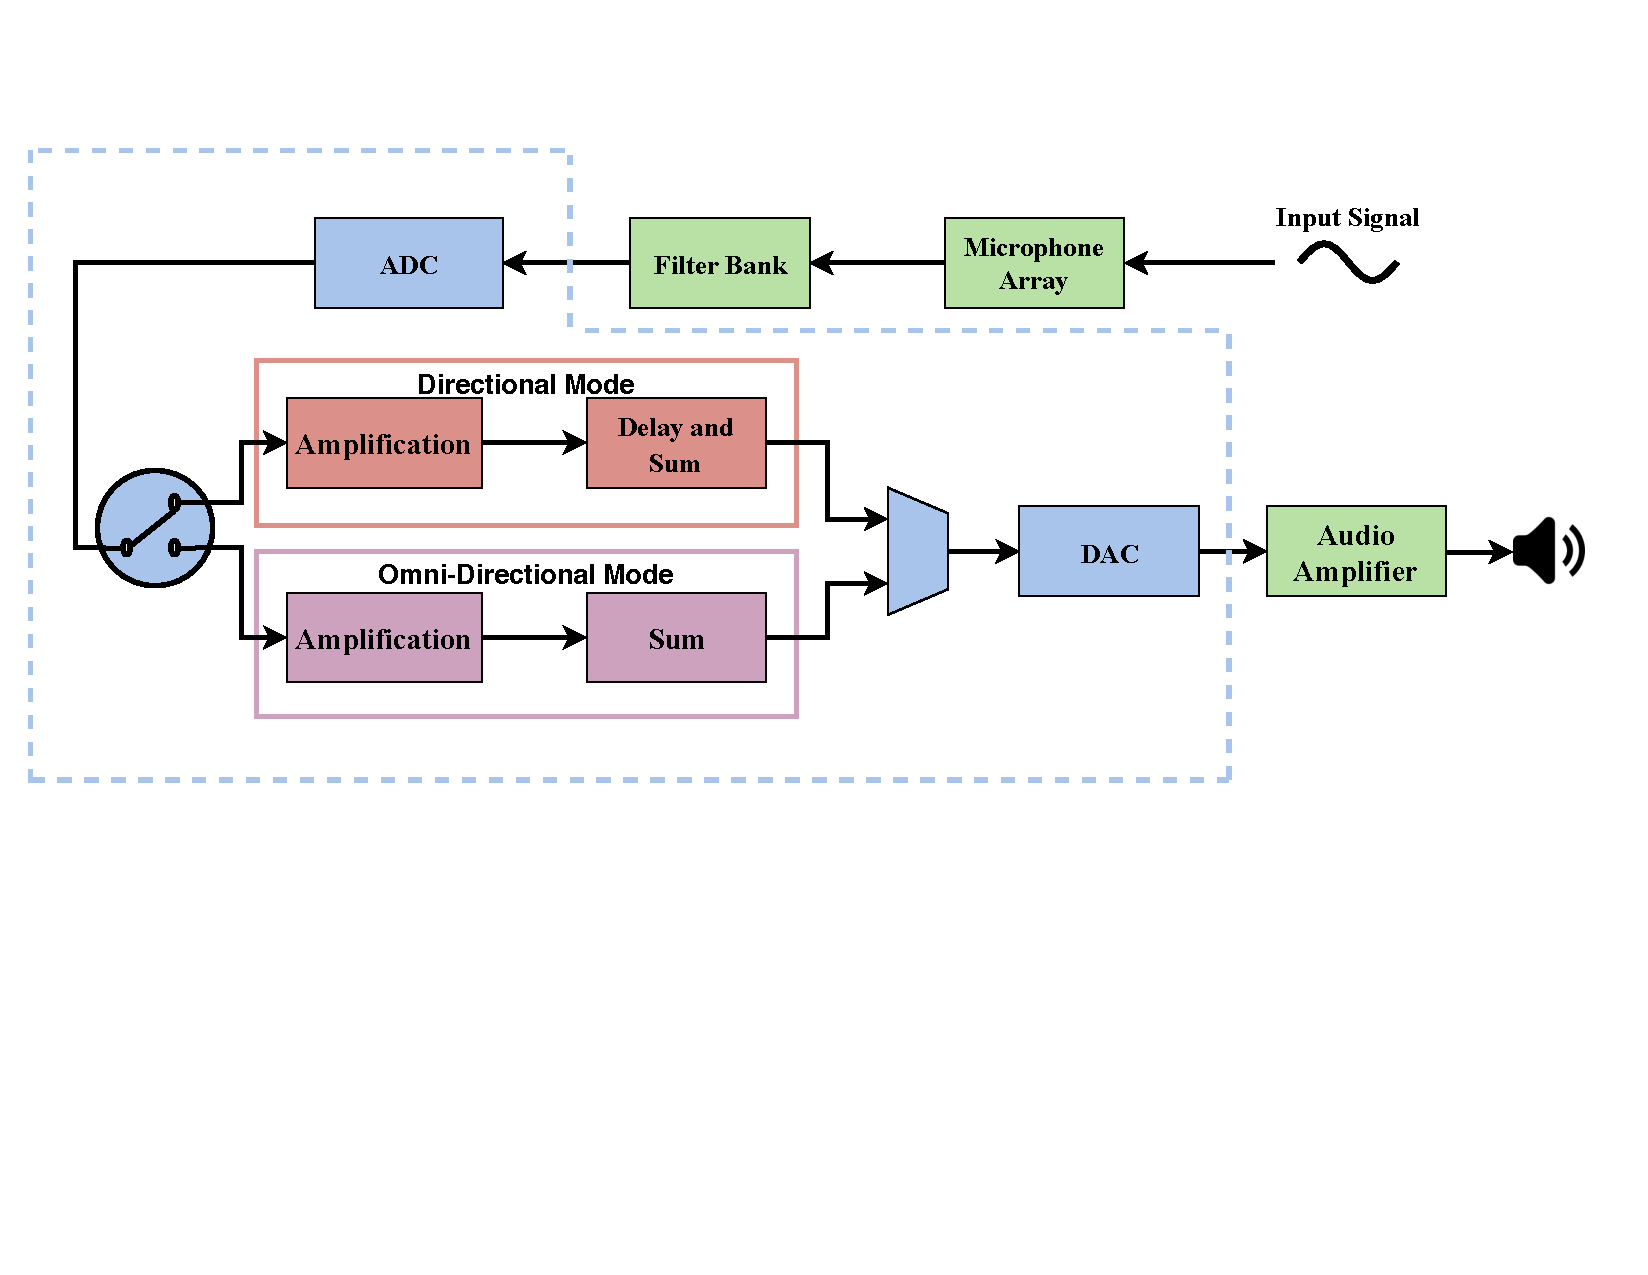
\includegraphics[width=1\linewidth]{posterBlockDiagram.pdf}
	\captionof{figure}{Hearing aid system overview}
\end{center}

{\large \textbf{Simulated vs Hardware Hearing Aid}}
	\vspace{-1em}
\begin{center}
\captionof{table}{Comparison of simulated and hardware hearing aids}
	\resizebox{\columnwidth}{!}{%
\begin{tabular}{ccc}
\toprule
	\textbf{Property} & \textbf{Simulation} & \textbf{Hardware} \\ 
\midrule
	Number of Microphones & 10 & 4 \\ 

	Bandwidth & 0.25-8~kHz & 2.8-3.5kHz and 5.6-7~kHz \\ 

	Filter order & 14 & 2 \\ 

	Type of filters & $\frac{1}{3}$ Octave bandpass & $\frac{1}{3}$ Octave bandpass \\ 

	Number of filters & 16 per microphone & 2 per microphone \\ 
	Number of steerable angles & 19 (${10}^o$ increments) & 5 (${0}^o$, ${60}^o$, ${90}^o$, ${120}^o$, ${180}^o$) \\ 
\bottomrule
\end{tabular} 
}
\end{center}

{\large \textbf{Device Testing}}
\begin{center}
	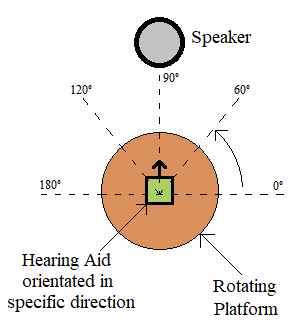
\includegraphics[width=0.4\linewidth]{directionalityLabTest.png}
	\captionof{figure}{Procedure for testing the hearing aid}
\end{center}
}


%----------------------------------------------------------------------------------------
%	CONCLUSION
%----------------------------------------------------------------------------------------

\headerbox{Conclusion}{name=conclusion,column=2,below=FutureWork}{ % This block's bottom aligns with the bottom of the conclusion block
This project is a proof of concept that an inexpensive, fully functional, adaptive hearing aid can be produced. Amplification to to specific frequency bands in accordance with provided audiograms can be achieved. Additionally, it is possible to achieve directionality in hearing aid devices by utilizing array theory. The total cost to construct the device is R1500. 
	\item Amplification to to specific frequency bands in accordance with provided audiograms can be achieved
	\item Achieving directionality in hearing aid devices is possible by utilizing array theory
	\item The total cost to construct the device is R1500 
	\item Average error between simulated and measured beam steering = 32.9\% 
	\item Average error with respect to	
}

%----------------------------------------------------------------------------------------
%	REFERENCES
%----------------------------------------------------------------------------------------

\headerbox{References}{name=references,column=2,above=bottom, below=conclusion}{
	
	\renewcommand{\section}[2]{\vskip 0.05em} % Get rid of the default "References" section title
	\nocite{*} % Insert publications even if they are not cited in the poster
	\small{ % Reduce the font size in this block
		\bibliographystyle{unsrt}
		\bibliography{sample} % Use sample.bib as the bibliography file
}}

%----------------------------------------------------------------------------------------
%	RESULTS
%----------------------------------------------------------------------------------------

\headerbox{Results: Simulation}{name=results,column=1,row=0}{

In the figure below, the frequency spectrum of the output from the hearing aid is compared to that of the original signal so that the effects of compensatory amplification can be seen
\begin{center}
	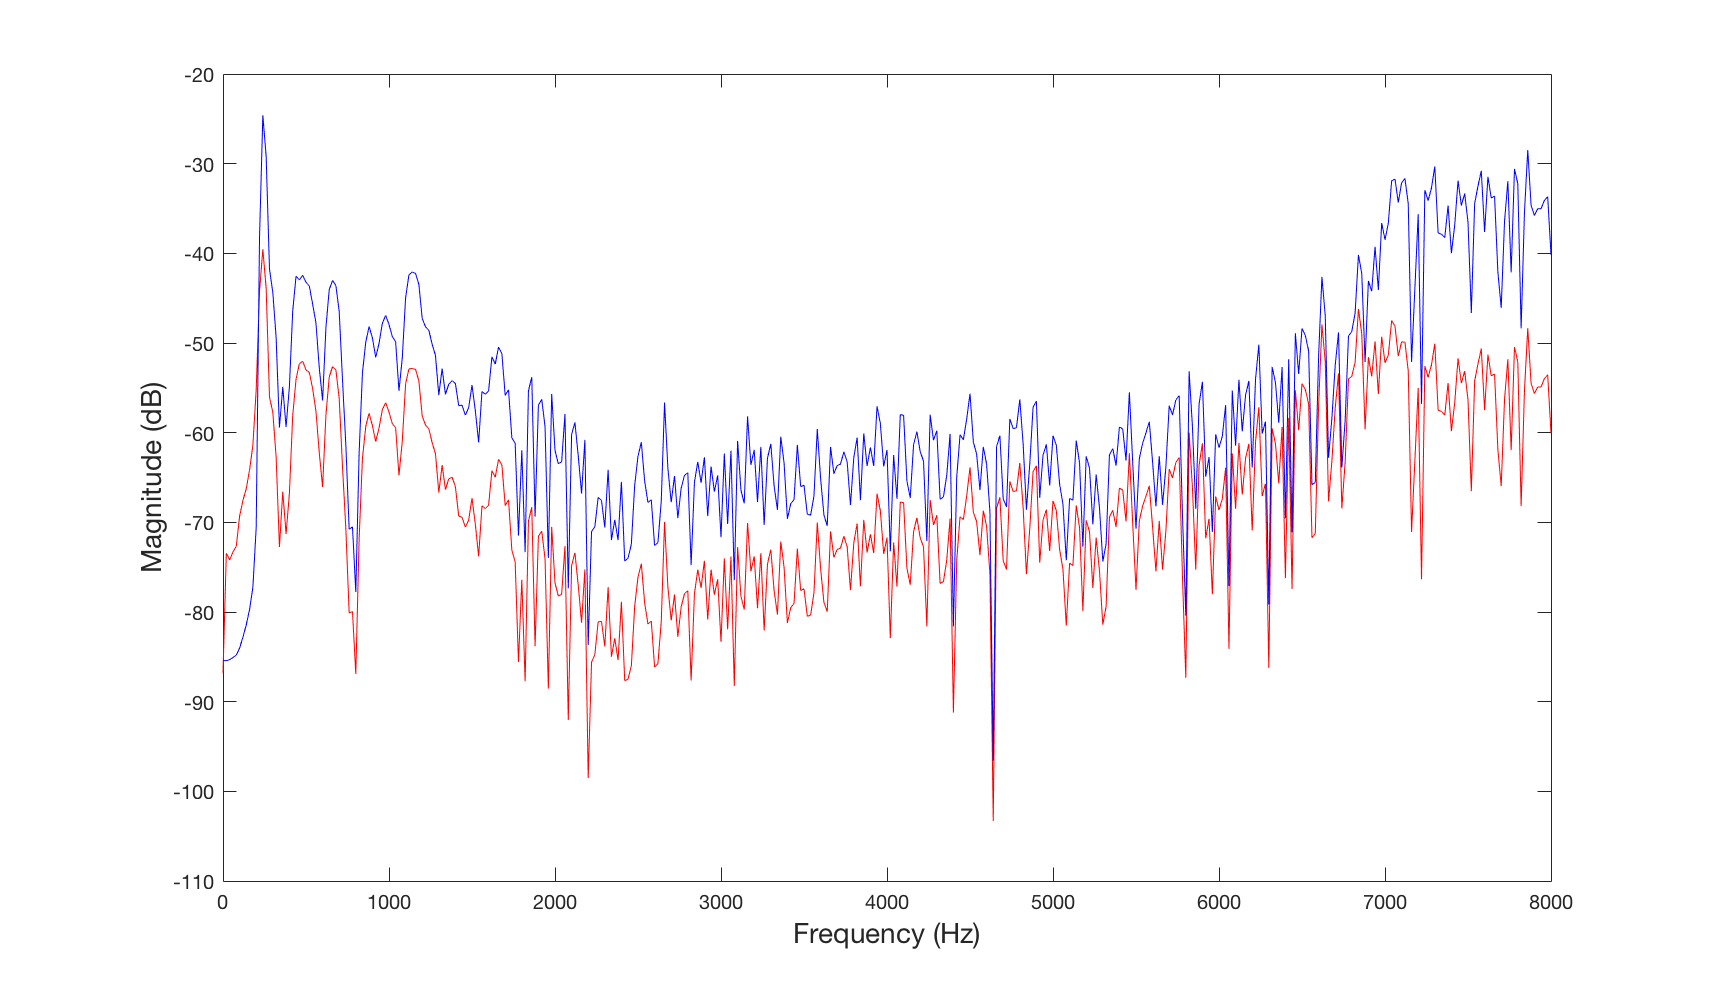
\includegraphics[width=0.6\linewidth]{fftSoftware.png}
	\captionof{figure}{FFT of the input signal and the output signal from the hearing aid}
\end{center}

The polar plot shows the normalised magnitudes of the signal at various angles, with respect to the user, when the dial is facing $90^{o}$
	\begin{center}
	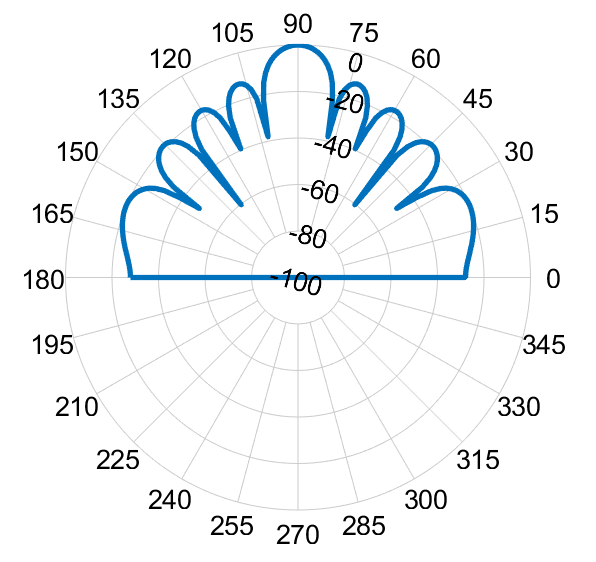
\includegraphics[width=0.3\linewidth]{polar90degSoftware.png}
	\captionof{figure}{Gain applied to the output signal when the beam is steered to ${90}^o$}
\end{center}

}
%------------------------------------------------
\headerbox{Results: Hardware}{name=results2,column=1, bottomaligned=references, below=results}{
%\begin{multicols}{2}
%	\vspace{1em}
The effects of compensatory gain are illustrated below through the application of different amplifications to the two frequency bands
	\begin{center}
		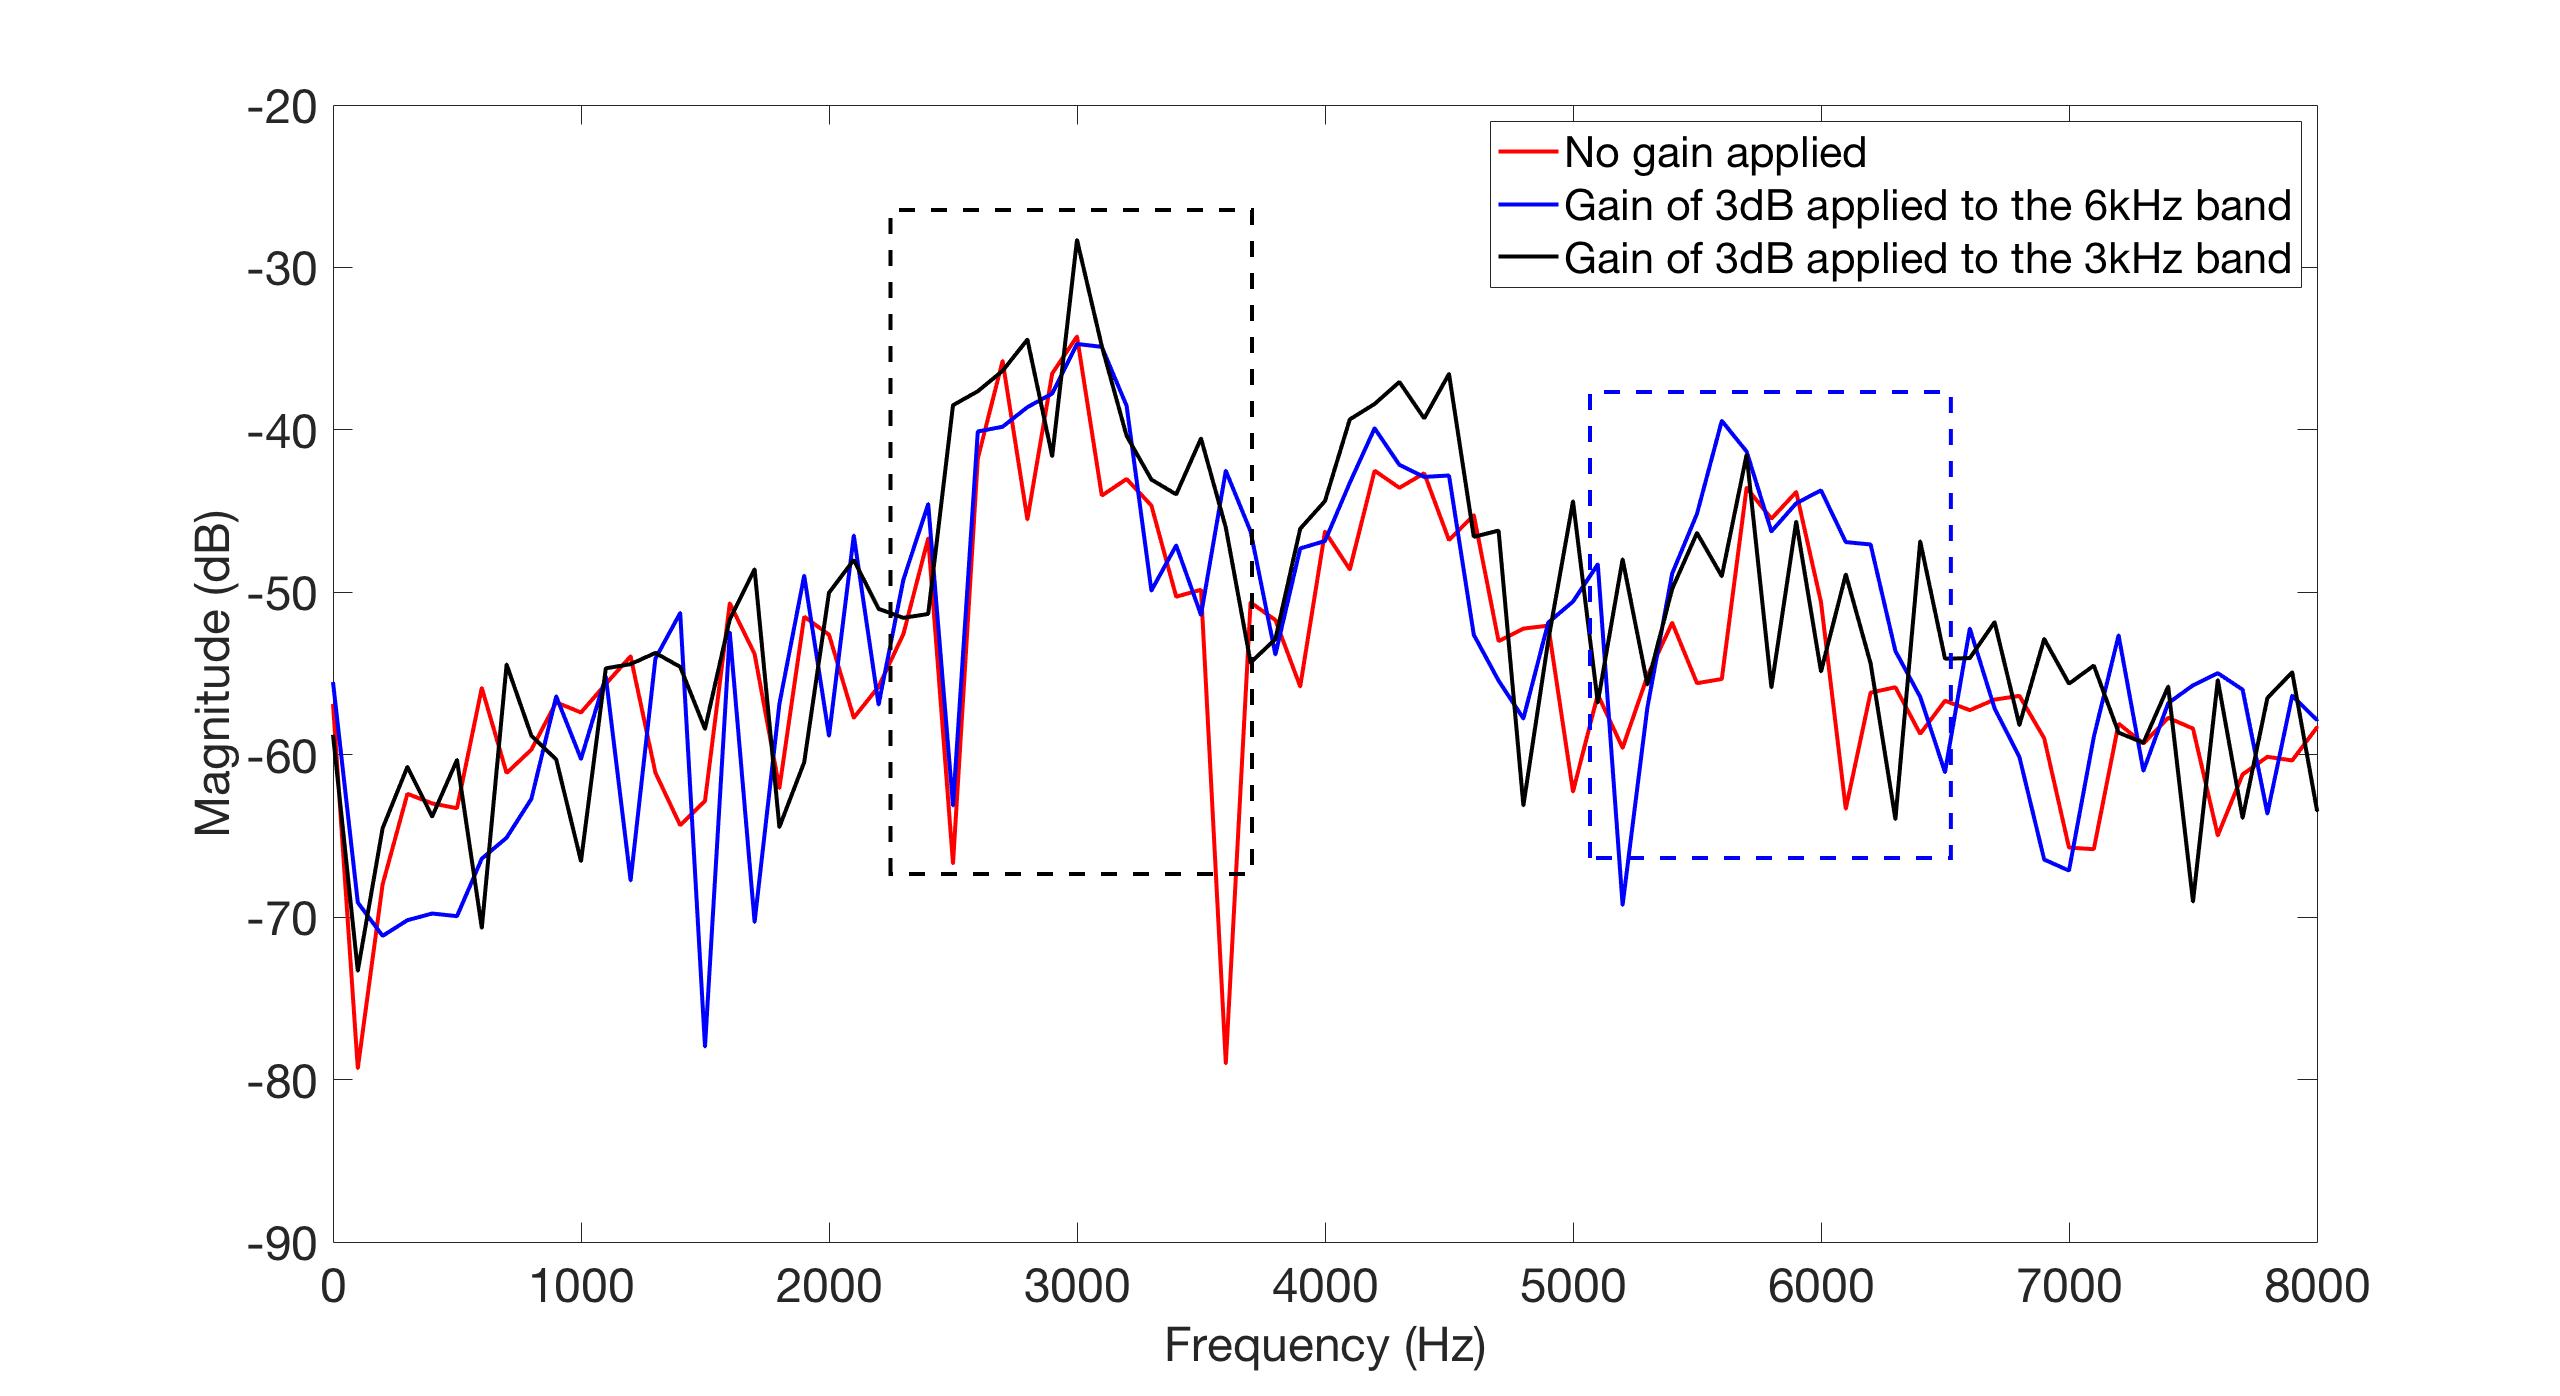
\includegraphics[width=0.6\linewidth]{hardwareGain.png}
		\captionof{figure}{FFT of the output signal from the hearing aid with various amplifications}
	\end{center}

A simulated response was created using 4 microphones. This response was compared to the measured response acquired during device testing
	\begin{center}
		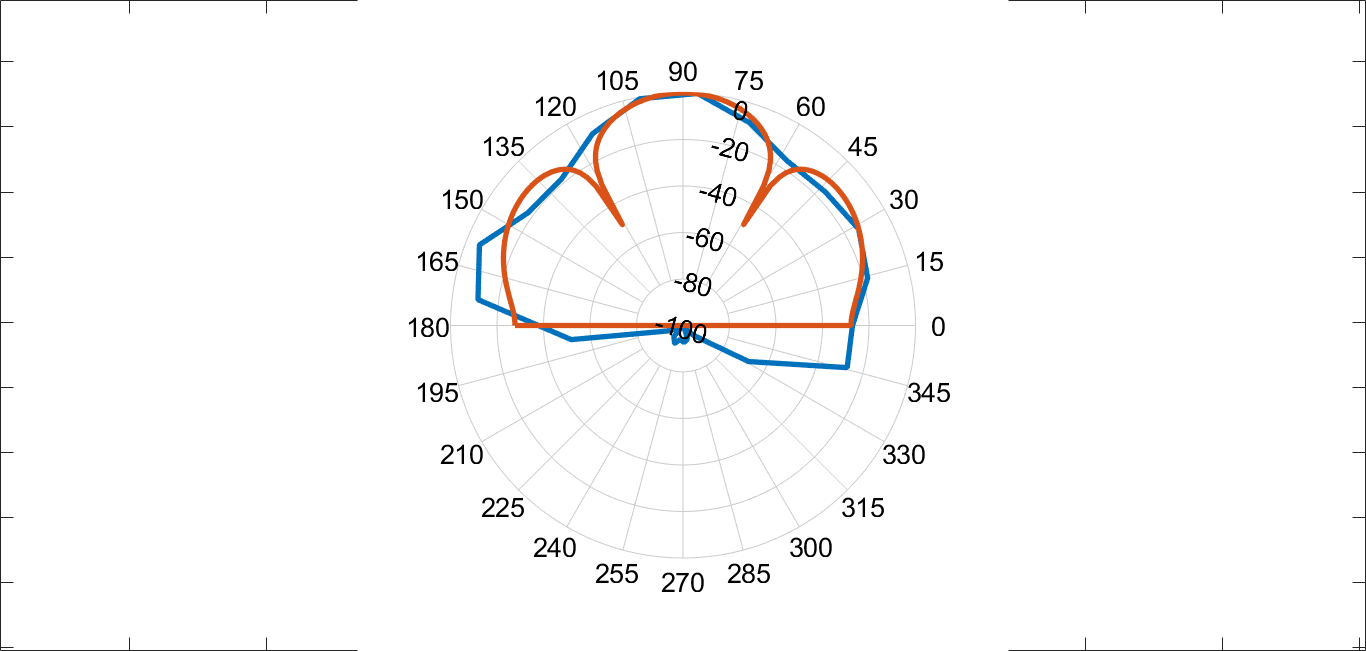
\includegraphics[width=0.3\linewidth]{deg90hardware.png}
		\captionof{figure}{Gain applied to the output signal when the beam is steered to ${90}^o$}
	\end{center}

	
%\end{multicols}
}


%----------------------------------------------------------------------------------------

\end{poster}

\end{document}